\documentclass[aspectratio=1610,12pt,xcolor=dvipsnames]{beamer}
\mode<presentation>

% Respect chosen fonts (serif) and metrics
\usefonttheme{professionalfonts}
\renewcommand{\familydefault}{\rmdefault}

% Figures
\usepackage{graphicx}
\usepackage{float}

%% table
\usepackage{xcolor}
\usepackage{fancyhdr}
\usepackage{booktabs}
\usepackage[table]{xcolor}

% subsection page template
\setbeamertemplate{subsection page}
{
  \begin{centering}
    \vfill
    {\usebeamerfont{section title}\usebeamercolor[fg]{section title}\Large\insertsubsectionhead\par}
    \vfill
  \end{centering}
}
% section page template
\setbeamertemplate{section page}
{
  \begin{centering}
    \vfill
    {\usebeamerfont{section title}\usebeamercolor[fg]{section title}\Large\insertsectionhead\par}
    \vfill
  \end{centering}
}

%% footnote
\setbeamertemplate{footnote}{%
  \parindent 0em\noindent%
  \raggedright\insertfootnotemark\insertfootnotetext\par%
}

%% theme
\usetheme{default}
\useoutertheme{miniframes}
\definecolor{nagivation}{rgb}{0,0,0.35} % (typo kept if intentional)
\definecolor{main}{rgb}{0,0,0.5}
\setbeamercolor{structure}{bg=white,fg=nagivation}
\setbeamercolor{frametitle}{fg=nagivation}
\setbeamercolor{section in head/foot}{fg=white,bg=nagivation}
\setbeamertemplate{footline}[page number]
\setbeamertemplate{items}[circle]
\setbeamerfont{footnote}{size=\footnotesize}
\setbeamerfont{caption}{size=\footnotesize}
\setbeamertemplate{subsection in head/foot}{}%
\setbeamertemplate{subsection in head/foot shaded}{}%

%% font
\usepackage{dsfont}
\usepackage{newpxtext}
\usepackage{newpxmath}
\usepackage{amsmath}

% Math & bib
\usepackage{amsmath,amsfonts,amssymb,bm}
\DeclareMathOperator*{\argmin}{arg\,min}
\newcommand{\indep}{\perp\!\!\!\, \perp}
\usepackage{natbib}
\bibliographystyle{asr}
\setcitestyle{aysep={}}
\usepackage[english]{babel}

\makeatletter
\DeclareRobustCommand\citep
{\begingroup\scriptsize\color{gray}\NAT@swatrue\let\NAT@ctype\z@\NAT@partrue
    \@ifstar{\NAT@fulltrue\NAT@citetp}{\NAT@fullfalse\NAT@citetp}}
\makeatother

% Roman numerals macro
\newcommand{\rom}[1]{\uppercase\expandafter{\romannumeral #1\relax}}

%% Title
\title[CML]{SOC 690S: Machine Learning in Causal Inference\\[1.5pt]}
\subtitle{\large Week 4: Neyman Orthogonality and Causal Inference Basics\\[-10pt]}

%% author
\author[Jiang] 
{\large Wenhao Jiang\vspace{-2em}}

%% affiliation
\institute[Duke]{}
\titlegraphic{
\includegraphics[height=1.4cm]{Misc/duke_logo.png}}

\date[Duke]
{\large Department of Sociology, Fall 2025}

\begin{document}

%%%%%%%%%%%%%%%%%%%%%%%%%%%%%%%%%%%%
%%%%%%%%Begin Main Content%%%%%%%%%%
%%%%%%%%%%%%%%%%%%%%%%%%%%%%%%%%%%%%

%% Title page %%
\begin{frame}
    \titlepage 
\end{frame}

\section{Neyman Orthogonality}

\begin{frame}
  \sectionpage
\end{frame}

\begin{frame}{Why do we need Neyman Orthogonality}
\begin{itemize}
    \item We want to estimate a causal effect of a treatment $D_i$ on an outcome $Y_i$
    \item One problem that is central to our course is that there is a high-dimensional set of controls $X_i$ that confound $D_i$ and $Y_i$
    \item Ordinary regression becomes problematic when $X_i$ is large in dimension or is highly nonlinear \pause
    \item We borrowed the insight from the \textit{Frisch-Waugh-Lovell} (FWL) theorem and produce estimate of $Y_i$ and $D_i$ based on $X_i$ using Machine Learning
    \item The justification of why such \textit{Double Machine Learning} technique works is the \textit{Neyman Orthogonality}
    \item There are other methods, such as \textit{Augmented Inverse Propensity Weighting}, that do not rely on the particular form of \textit{double partialling out} but satisfy \textit{Neyman Orthogonality}
\end{itemize}
\end{frame}

\begin{frame}{The Structural Model}
\begin{itemize}
    \item Assume the following structural equation in the \textit{population}, where the causal effect of $D_i$ on $Y_i$ is well defined:
    \[
    Y_i = \theta_0 D_i + g_0(X_i) + \epsilon_i, 
    \quad E[\epsilon_i|D_i,X_i]=0
    \]
    \item $\theta_0$: parameter of interest (causal effect of $D_i$)
    \item $g_0(X_i)$: nuisance function capturing the effect of $X_i$ on $Y_i$ net of $D_i$
    \item $\epsilon_i$: error term, mean zero conditional on $D_i, X_i$
    \item Note that $g_0(X_i) \neq E[Y_i|X_i]$
    \[
    E[Y_i|X_i] = \theta_0 m_0(X_i) + g_0(X_i),
    \quad m_0(X_i) = E[D_i|X_i]
    \]
\end{itemize}
\end{frame}


\begin{frame}{Normal Equation from the Structural Model}

\begin{itemize}
    \item Define residualized treatment:
    \[
    \tilde D_i = D_i - m_0(X_i), \quad m_0(X_i)=E[D_i|X_i]
    \]
    \item Define residualized outcome (structural)
    \[
    \tilde Y_i = Y_i - g_0(X_i)
    \]
    \item \textit{Population} normal equation
    \[
    E\big[(\tilde Y_i - \theta_0 \tilde D_i)\tilde D_i\big] = 0
    \]
    \item This identifies $\theta_0$ under exogeneity
\end{itemize}
\end{frame}

\begin{frame}{Equivalence with FWL Residualization}

\begin{itemize}
    \item By the \textit{Frisch-Waugh-Lovell} (FWL) theorem, we can also residualize using conditional expectation:
    \[
    \tilde Y_i = Y_i - E[Y_i|X_i], 
    \quad \tilde D_i = D_i - E[D_i|X_i]
    \]
    \item The \textit{population} normal equation is
    \begin{align*}
      E[(Y_i - E[Y_i|X_i] - \theta_0(D_i -m_0(X_i)))\cdot (D_i -m_0(X_i)] &= 0 \\
      E[(Y_i - g_0(X_i) - \theta_0m_0(X_i) - \theta_0(D_i -m_0(X_i)))\cdot (D_i -m_0(X_i)] &= 0 \\
      E\big[(\tilde Y_i - \theta_0 \tilde D_i)\tilde D_i\big] &= 0
    \end{align*}
    \item FWL residualization and the structural model lead to the \textit{same normal equation}
\end{itemize}
\end{frame}

\begin{frame}{The Score Function}

\begin{itemize}
    \item Generalize to generic \textit{nuisance functions} $g(\cdot), m(\cdot)$
    \[
    \tilde Y_i = Y_i - g(X_i), 
    \quad \tilde D_i = D_i - m(X_i)
    \]
    \item Define the \textit{score function} that is analogous to the \textit{normal equation} based on the FWL theorem
    \[
    \psi(W_i; \theta, g, m) = 
    (Y_i - g(X_i) - \theta(D_i - m(X_i)))(D_i - m(X_i))
    \]
    \item $\theta_0$ can be identified with moment condition satisfying
    \[
    E[\psi(W_i; \theta_0, g, m)] = 0
    \quad \text{where } g=E[Y|X],\, m=E[D|X]
    \]
    \item We write $\psi(W_i; \theta, g, m)$ as $\psi(W_i; \theta, \eta)$ where $\eta = (g,m)$ 
\end{itemize}
\end{frame}

\begin{frame}{Moment Function and Neyman Orthogonality}
\begin{itemize}
    \item Formally, moment condition is defined as
    \[M(\theta, \eta) = E[\psi(W; \theta, \eta)]\]
    \item At the true nuisances $\eta = \eta_0$ ($g_0$ and $m_0$ correctly specified), the moment condition has a unique root at $\theta_0$; that is
    \begin{align*}
        M(\theta, \eta_0) = 0 \text{ if and only if } \theta=\theta_0
    \end{align*}
    \item Remember in the \textit{structural equation}, $g_0(X_i)$ is defined as the effect of $X_i$ on $Y_i$ \emph{net of $D_i$}
    \item In practice, replace $g_0(X_i)$ by $g(X_i) = E[Y_i|X_i]$ produces the same \textit{normal equation} and identify the same $\theta_0$
\end{itemize}
\end{frame}

\begin{frame}{Moment Function and Neyman Orthogonality}

\begin{itemize}
    \item In reality, we do not know the true \textit{nuisance functions}
    \[
    g_0(X_i) = E[Y_i|X_i], \quad m_0(X_i) = E[D_i|X_i]
    \]
    \item We can only approximate them using \textit{finite samples} and \textit{predictive} methods
    \item The key idea is that we want estimation errors in $\hat \eta$ to have minimal impact on $\hat\theta$
    \item \textit{Neyman Orthogonality:} the score $\psi$ is \textit{Neyman orthogonal} if
    \[
    \partial_\eta M(\theta_0,\eta)\Big|_{\eta=\eta_0} = 0
    \]
    \item It means that the slope of $M$ in the \textit{nuisance} direction is flat at the truth
    \item If we plug in $\hat \eta$ that is close to $\eta_0$, the bias in the estimation of $M$ and the associated \textit{normal equation} is only \textit{second order}, not first order
\end{itemize}
\end{frame}

\begin{frame}{Neyman Orthogonality via Gateaux Derivative}

\begin{itemize}
    \item Gateaux derivative is the functional derivative
    \begin{align*}
    \partial_g M(\theta_0,g,m_0)[\Delta]\;\Big|_{g=g_0} 
    &= \lim_{t \to 0} \frac{M(\theta_0,g_0+t\Delta,m_0) - M(\theta_0,g_0,m_0)}{t} \\
    M(\theta_0,g_0 + t\Delta,m_0) 
    &= E\Big[(Y_i - g_0(X_i) - t \Delta(X_i) - \\ &\hspace{2.5em} \theta_0(D_i-m_0(X_i)))(D_i-m_0(X_i))\Big] \\
    &= M(\theta_0,g_0,m_0) - t E[\Delta(X_i)(D_i-m_0(X_i))] \\
    \partial_g M(\theta_0,g,m_0)[\Delta]\;\Big|_{g=g_0} 
    &= -E[\Delta(X_i)(D_i-m_0(X_i))]
    \end{align*}
    \item Since $E[D_i-m_0(X_i) | X_i]=0$, this expectation is zero for all directions $\Delta$ (\textit{CEF Decomposition Property})
    \item By symmetry, the derivative \textit{w.r.t.} $m$ also vanishes at $(g_0,m_0)$
    \item The gradient of $M(\theta_0,\eta)$ with respect to $\eta=(g,m)$ is \textit{0 at the truth}
\end{itemize}
\end{frame}


%=========================================================

\begin{frame}{Taylor Expansion of the Moment Function}

\begin{itemize}
    \item Expand around the true nuisances $\eta_0=(g_0,m_0)$ using Taylor Expansion
    \begin{align*}
M(\theta_0,\hat\eta)
    &\approx M(\theta_0,\eta)\Big|_{\eta=\eta_0} + \underbrace{\left[\partial_\eta M(\theta_0,\eta)\Big|_{\eta=\eta_0}\right](\hat\eta-\eta_0)}_{\text{first order vanishes}} \\
    &+ 1/2(\hat\eta-\eta_0)'\left[\partial^2_\eta M(\theta_0,\eta)\Big|_{\eta=\eta_0}\right](\hat\eta-\eta_0) + \textit{ higher order}
    \end{align*}
    \item \textit{Without orthogonality}, the first-order term drives bias
    \item \textit{With orthogonality}, the first-order term vanishes, and the remaining error is mainly \textit{second-order} in 
    $(\hat\eta-\eta_0)$
    \item With Neyman orthogonality, it suffices for the nuisance estimates to converge at rate faster than $n^{1/4}$, rather than the much stronger $n^{1/2}$ rate that is generally impossible in high dimensions
\end{itemize}
\end{frame}

\begin{frame}{Heuristic Geometric Representation}
\begin{itemize}
    \item Think of the moment function
    \[
    M(\theta_0,g,m) = E[\psi(W;\theta_0,g,m)]
    \]
    as a \textit{surface} over the nuisance directions $(g,m)$
    \item If the functional gradient \textit{w.r.t.} $(g,m)$ is nonzero,
    the surface is \textit{tilted}; small errors in $(\hat g,\hat m)$
    shift the zero point and bias the estimation of $\theta_0$
    \item If the gradient is zero (\textit{orthogonality}),
    the surface is \textit{flat} in nuisance directions at the truth;
    $\theta_0$ is robust to small nuisance estimation error
\end{itemize}
\end{frame}

\begin{frame}{Orthogonal vs. Non-Orthogonal Surfaces}
\begin{figure}
    \centering
    \hspace*{-1.6cm} % shift left
    \vspace*{2em} % shift up
    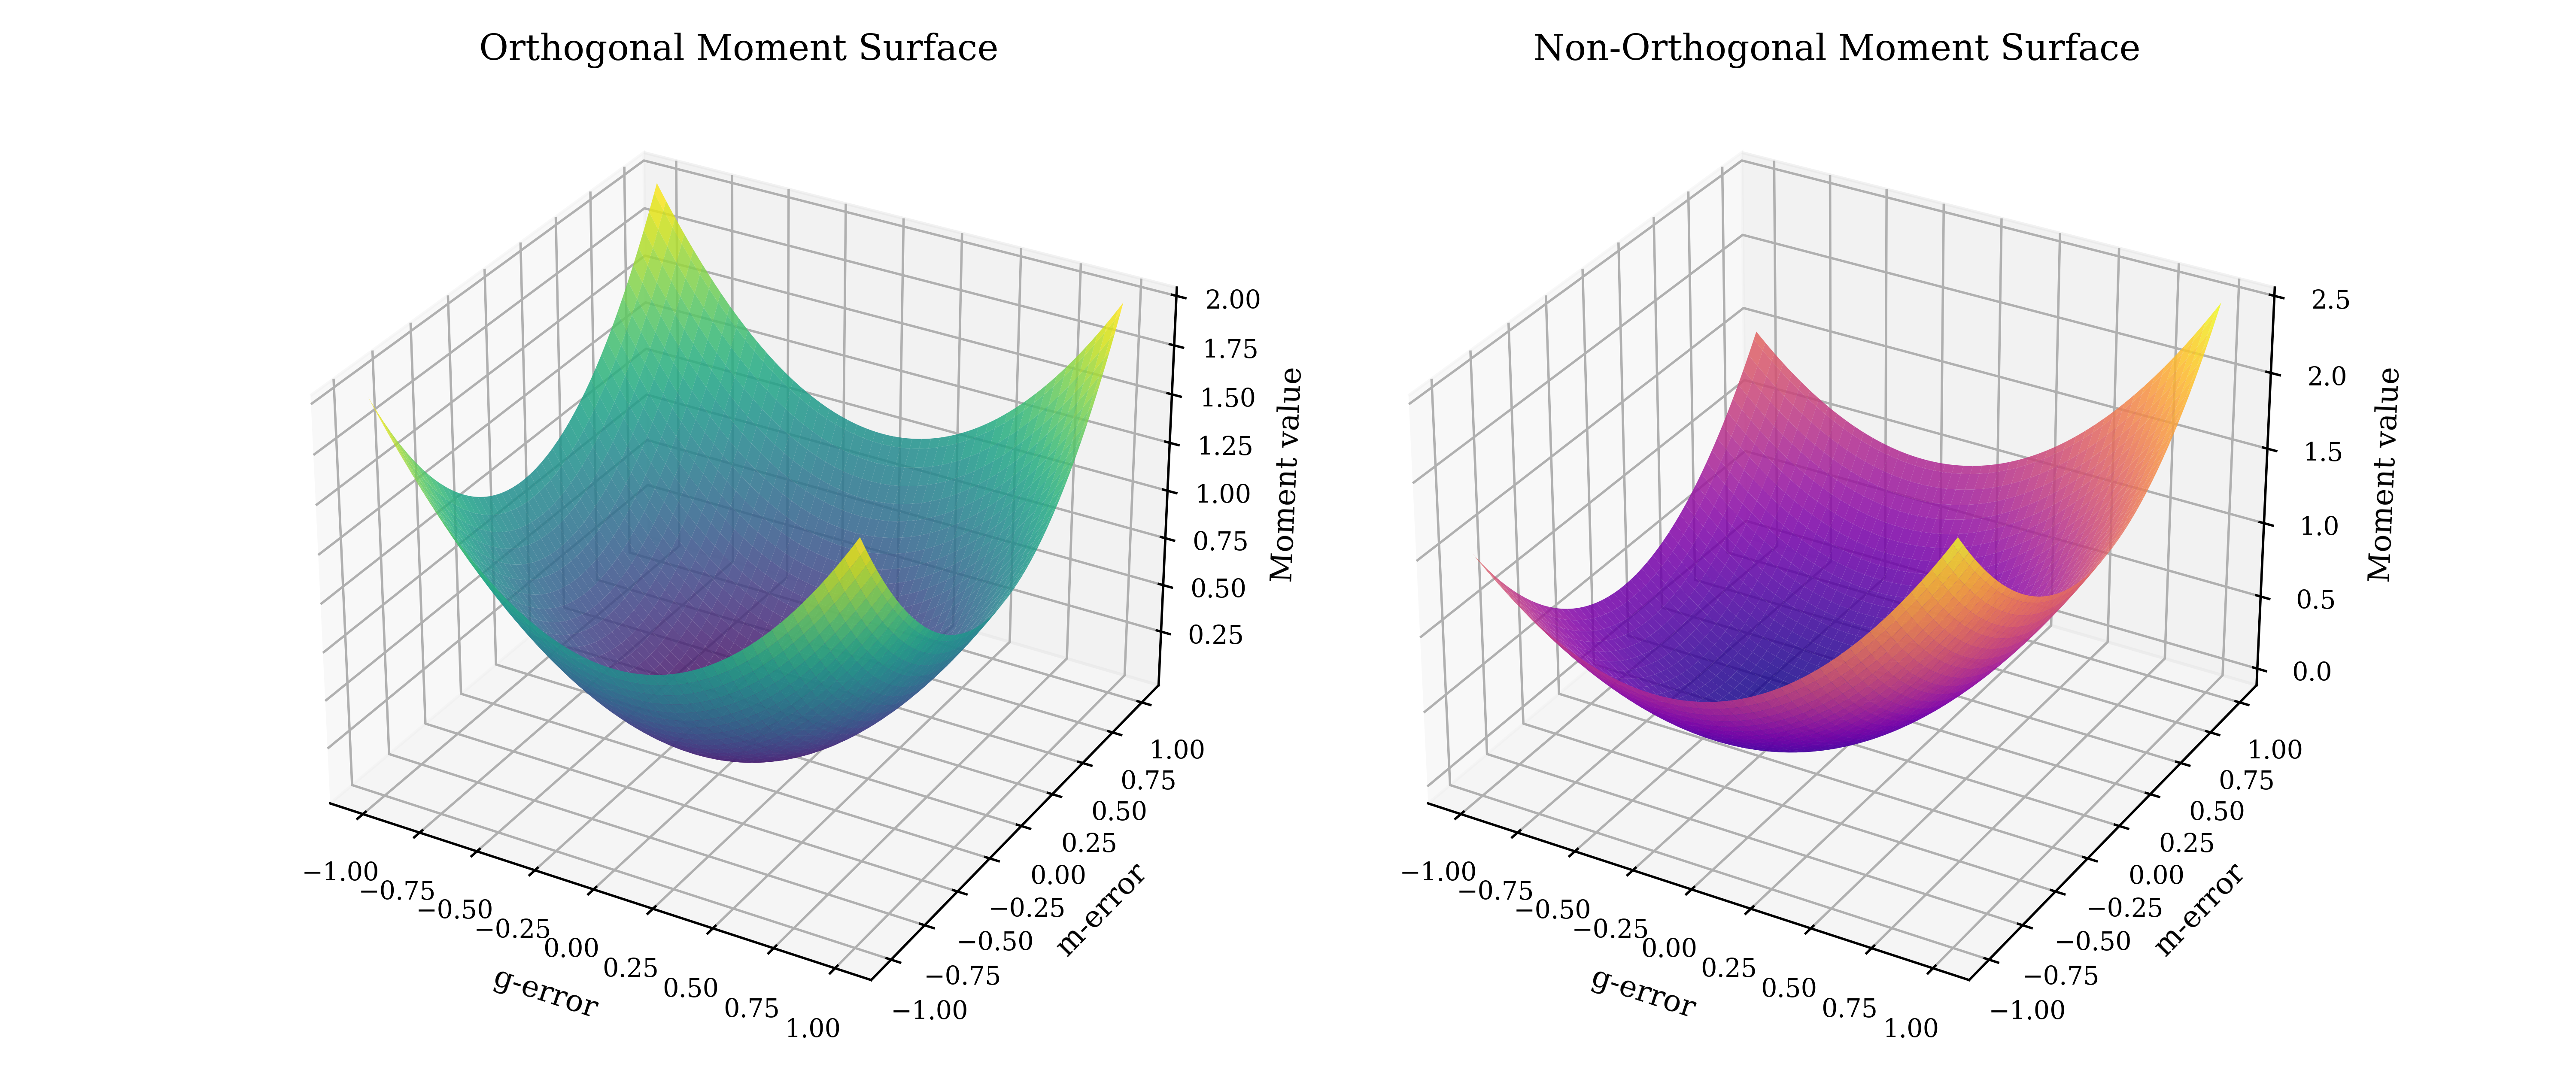
\includegraphics[width=1.15\linewidth]{Causal Inference Basics/Figures/orthogonal vs. non.png}
\end{figure}
\end{frame}

\subsection{Double Machine Learning}

\begin{frame}
  \subsectionpage
\end{frame}

\begin{frame}{Invalid Single LASSO Estimation (Naive Method)}

\begin{itemize}
    \item We mentioned in Week 2 that an intuitive but incorrect LASSO estimator only does LASSO once (\textit{Neyman Orthogonality} not satisfied)
    \item One applies LASSO regression of $Y_i$ on $D_i$ and $X_i$ to select relevant covariates $X_Y$, in addition to the covariate of interest, then refits the model using OLS of $Y_i$ on $D_i$ and $X_Y$
\end{itemize}
\end{frame}

\begin{frame}{Why Single LASSO Fails}
\begin{itemize}
    \item The implicit \textit{score function} 
    \[
    \psi^{naive}(W_i;\theta,g) = (Y_i - g(X_i) - \theta D_i)D_i
    \]
    where $g(X_i)$ captures the effect of selected controls $X_Y$
    \item \textit{Population} moment is defined as
    \[
    M^{naive}(\theta,g) = E[\psi^{naive}(W_i;\theta,g)]
    \]
    \item With Gateaux derivative \textit{w.r.t.} $g$ in direction $\Delta$:
    \begin{align*}
    \partial_g M(\theta_0,g)[\Delta]\;\Big|_{g=g_0}
  &= -E[\Delta(X_i)D_i] \\ 
  &= -E[E[\Delta(X_i)D_i|X_i]] \\
  &= -E[\Delta(X_i) E[D_i|X_i]] \neq 0
    \end{align*}
    \item \textit{Neyman orthogonality} fails; bias in $\hat g$ contaminates $\hat \theta$ at first order
\end{itemize}
\end{frame}

\begin{frame}{Double LASSO}

\begin{itemize}
    \item Remember Double LASSO satisfies \textit{Neyman Orthogonality}
    \item With Gateaux derivative \textit{w.r.t.} $g$ in direction $\Delta$:
    \begin{align*}
    \partial_g M(\theta_0,g,m_0)[\Delta]\;\Big|_{g=g_0}
  &= -E[\Delta(X_i)(D_i - m_0(X_i)]
    \end{align*}
    \item Under \textit{approximate sparsity}, LASSO can consistently approximate $m_0(X_i)$ at rate $\geq n^{1/4}$ in high dimension
    \begin{align*}
        -E[\Delta(X_i)(D_i - m_0(X_i)] &= \\
        -E[E[\Delta(X_i)(D_i - m_0(X_i)|X_i]] &= 0
    \end{align*}
    \item In actual estimation, we use \textit{plug-in} method to fine-tune \textit{penalty level} $\lambda$ to find a good approximation to the \textit{nuisance functions} $m_0(X_i)$ (and $g_0(X_i)$)
\end{itemize}
\end{frame}

\begin{frame}{Double Machine Learning}

\begin{itemize}
    \item Similar to Double LASSO, when we use other Machine Learning methods,
    we need to \textit{fine-tune hyperparameters} (penalty level, tree depth, or neural network size)
    to strike the \textit{bias-variance tradeoff} and obtain consistent estimations of the
    \textit{nuisance functions}
    \[
    m_0(X) = E[D|X], \quad g_0(X) = E[Y|X]
    \]
    \item But Double Machine Learning adds an another essential step of \textit{cross-fitting}
\end{itemize}
\end{frame}

\begin{frame}{Double Machine Learning: Cross-Fitting}

\begin{itemize}
    \item Instead of predicting the \textit{nuisance functions} based on the full \textit{sample}
    \item We only train nuisance models on $K-1$ folds, and predict the \textit{residualized} $Y_i$ and $D_i$ on the held-out fold $k$
    \item We stack predicted \textit{residualized} $Y_i$ and $D_i$ across $K$ folds and for our FWL estimator
    \item to form the \textit{score function} precisely to \textit{prevent overfitting}—we do not want to use the training data to predict its own nuisance function
    \item It ensures nuisance errors are \textit{out-of-sample}, so Neyman orthogonality cancels first-order bias
\end{itemize}
\end{frame}

\begin{frame}{Cross-Fitting and Moment Estimation}

\begin{itemize}
    \item The above intuitive steps can be formally expressed in moment condition
    \item We take a $K$-fold random partition $(I_k)_{k=1}^{K}$ of observation indices $\{1,...,n\}$ such that the size of each fold is about the same
    \item For each $k \in \{1,...,K\}$, construct a fine-tuned nuisance estimator $\hat \eta_{[k]}$ that depends on the subset of data that excludes the $k$-th fold
    \item Now let $k(i) = \{k:i \in I_k\}$, the \textit{sample} estimate of the moment equation is then defined as
    \[
    \hat M(\theta,\hat\eta) = \frac{1}{n}\sum_{i=1}^n 
    \psi\left(W_i;\theta,\hat \eta_{[k(i)]}\right)
    \]
    \item We find $\hat \theta$ by solving $\hat M(\hat\theta,\hat\eta)=0$
\end{itemize}
\end{frame}

\begin{frame}{Sandwich Variance Estimator}

\begin{itemize}
    \item Sandwich variance estimator is defined in the same fashion as before
    \begin{align*}
    \hat V &= \hat J^{-1}\hat \Omega \hat J^{-1} \\
    \hat J &= \frac{1}{n}\sum_{i=1}^n 
        \partial_\theta \psi(W_i;\hat\theta,\hat\eta) \\
    \hat \Omega &= \frac{1}{n}\sum_{i=1}^n 
        \psi(W_i;\hat\theta,\hat\eta)\,\psi(W_i;\hat\theta,\hat\eta)'
    \end{align*}
    \item This looks scary, but note that for the \textit{score function}
    \begin{align*}
    \psi(W_i;\theta,\eta) &= 
    (\tilde Y_i - \theta \tilde D_i)\tilde D_i \\
    \hat J = -\frac{1}{n}\sum_{i=1}^n \tilde D_i^2, &\quad
    \hat \Omega = \frac{1}{n}\sum_{i=1}^n 
    (\tilde Y_i - \hat\theta \tilde D_i)^2 \tilde D_i^2
    \end{align*}
\end{itemize}
\end{frame}

\begin{frame}{The Use of Cross-Fitting}

\begin{itemize}
    \item Remember the \textit{score function} is defined as
    \[
    \psi(W;\theta,\eta) = (Y_i - g(X_i) - \theta(D_i-m(X_i)))(D_i-m(X_i))
    \]
    \item Suppose we have a small estimation error in projecting $g_0$ and $m_0$
    \begin{align*}
    \hat g(X_i) &= g_0(X_i) + \delta_g(X_i), \quad 
    \hat m(X_i) = m_0(X_i) + \delta_m(X_i) \\
    \partial_g M(\theta_0,g,m)[\Delta]\;\Big|_{g=g_0} 
    &= -E[\delta_g(X_i)(D_i-\hat m_0(X_i))] \neq 0
    \end{align*}
     \item First-order bias terms does not vanish to 0 without \textit{cross-fitting}
     \item Using the whole sample to train nuisances breaks \textit{orthogonality}
\end{itemize}
\end{frame}

\begin{frame}{Double LASSO Does not Need Cross-Fit}

\begin{itemize}
    \item In general Double Machine Learning, \textit{nuisance functions} are estimated by flexible ML, and in-sample predictions can \textit{overfit}
    \item The nuisance errors $\delta_g(X_i),\delta_m(X_i)$ become correlated with residuals $D_i - m_0(X_i)$ \pause
    \item \textit{Nuisances} estimated by LASSO regression in a linear, approximately sparse setup
    \item Shrinkage bias is \textit{analytically controlled} by \textit{approximate sparsity}
    \item Correlation with residuals does not spoil inference
\end{itemize}
\end{frame}

\section{Potential Outcome Framework}

\begin{frame}
  \sectionpage
\end{frame}

\begin{frame}{Potential Outcomes Framework}
\begin{itemize}
\item For each unit \(i\), we fine two \textit{latent} variables  
  \begin{align*}
  &Y_i(1) \quad \text{(outcome if treated)} \\ \quad &Y_i(0) \quad \text{(outcome if not treated)} \\
  &Y_i(d) \quad d \in \{0,1\}
  \end{align*}
\item Individual treatment effect (ITE) is defined as  
  \[
  \tau_i = Y_i(1) - Y_i(0)
  \]
\item The fundamental problem of causal inference is that we cannot observe both \(Y_i(1)\) and \(Y_i(0)\) for the same unit
\item We define Average Treatment Effect (ATE) in the \textit{population} as 
  \[
  \delta = E[Y_i(1) - Y_i(0)] = E[Y_i(1)] - E[Y_i(0)]
  \]
\end{itemize}
\end{frame}

\begin{frame}{Average Predictive Effect and Selection Bias}
\begin{itemize}
\item Let \(D_i \in \{0,1\}\) denote \textit{actual} treatment assignment
\item The observed outcome is defined as
  \begin{align*}
  Y_i &= D_i Y_i(1) + (1 - D_i) Y_i(0)
  \end{align*}
  \item \textit{Population} data directly provide the conditional average
  \begin{align*}
  E[Y_i | D_i=1] &= E[Y_i(1) | D_i=1] \\
  E[Y_i | D_i=0] &= E[Y_i(0) | D_i=0]\\
  E[Y_i | D_i=d] &= E[Y_i(d) | D_i=d]  \quad d \in \{0,1\}
  \end{align*}
\end{itemize}
\end{frame}

\begin{frame}{Average Predictive Effect and Selection Bias}
\begin{itemize}
    \item The average predictive effect (APE) is defined as the naive difference between $Y_i$ in the treated and control group
  \[
  \pi = E[Y_i \mid D_i=1] - E[Y_i \mid D_i=0]
  \]
  \item If there is a \textit{selection bias}, APE $\pi$ will not agree with the ATE $\delta$ 
  \item Using potential outcomes, we want to decompose $\pi$
    \begin{align*}
    \pi &= E[Y_i \mid D_i=1] - E[Y_i \mid D_i=0] \\ 
    &= E[Y_i(1) \mid D_i=1] - E[Y_i(0) \mid D_i=0] \\
    &= \underbrace{\big(E[Y_i(1) \mid D_i=1] - E[Y_i(0) \mid D_i=1]\big)}_{\text{ATET}}
    + \\ &\hspace{2em} \underbrace{\big(E[Y_i(0) \mid D_i=1] - E[Y_i(0) \mid D_i=0]\big)}_{\text{Selection Bias}}
    \end{align*}
\end{itemize}
\end{frame}

\begin{frame}{Randomized Controlled Trials (RCT)}
\begin{itemize}
\item In a Randomized Controlled Trial (RCT), treatment is randomly assigned:  
  \begin{align*}
  D_i \indep (Y_i(0), Y_i(1)) &\quad \text{ or } D_i \indep Y_i(d) \\
  0 \leq P(D_i&=1) \leq 1  
  \end{align*}
\item The randomization of treatment assignment ensures that  
  \[
  E[Y_i \mid D_i=d] = E[Y_i(d) \mid D_i=d] = E[Y_i(d)]
  \]
\item The \textit{selection bias} term  
  \begin{align*}
      E[Y_i(0) \mid D_i=1] - E[Y_i(0) \mid D_i=0] = E[Y_i(0)] - E[Y_i(0)] = 0
  \end{align*}
  \item APE agrees with ATE
  \[
  \pi = E[Y_i \mid D_i=1] - E[Y_i \mid D_i=0] = \delta
  \]
\end{itemize}
\end{frame}

\begin{frame}{Statistical Inference with Two Sample Means}
\begin{itemize}
\item The APE is asymptotically normal in distribution
\item From an RCT, we collect \(\{(Y_i, D_i)\}_{i=1}^n\); we calculate the group means as 
  \[
  \hat{\theta}_d = \frac{\sum_{i=1}^n Y_i \cdot \mathds{1}(D_i = d)}{\sum_{i=1}^n \mathds{1}(D_i = d)}, \quad d \in \{0,1\}
  \]
\item APE agrees with ATE  
  \[
  \hat{\delta} = \hat{\theta}_1 - \hat{\theta}_0
  \]
\item APE and ATE is asymptotically normal under random assignment 
  \[
  \sqrt{n}(\hat{\delta} - \delta) \overset{d}{\to} N(0, \sigma^2) 
  \]
 \item If the treated and controlled observations are independent, variance is
\[
\sigma^2 = \frac{\operatorname{Var}(Y_i \mid D_i=1)}{P(D_i=1)} 
  + \frac{\operatorname{Var}(Y_i \mid D_i=0)}{P(D_i=0)}
\]
\end{itemize}
\end{frame}

\begin{frame}{Assumptions and Limitations of RCTs}
\begin{itemize} 
\item \textit{Ethical issues:} cannot randomize harmful treatments 
\item \textit{Practical challenges:} cost of RCTs can be high
\item \textit{External validity:} if experiment is localized, results may not generalize \pause
\item \textit{The Stable Unit Treatment Value Assumption (SUTVA)}: Treatment of one unit does not change outcomes of others; no spillover effect and no interference across units
\end{itemize}
\end{frame}

\subsection{Causal Inference via Conditional Ignorability}

\begin{frame}
  \subsectionpage
\end{frame}

\begin{frame}{Potential Outcome and Ignorability}

\begin{itemize}
    \item In reality, the complete random assignment assumption may be too strong
    \[D_i \indep Y_i(d)\]
    \item The treated and controlled units may differ in some characteristics $X_i$
    \item But with the same strata of $X_i$, treatments are as if randomly assigned
    \[D_i \indep Y_i(d) \mid X_i \]
    \item That is, suppose treatment status $D_i$ is independent of potential outcomes $Y_i(d)$ conditional on a set of covariates $X_i$—\textit{ignorability} assumption
    \item We also assume that there is \textit{overlap} or \textit{full support} in the distribution of probability of receiving treatment by $X_i$
    \begin{align*}
        p(X_i) &:= P(D_i=1|X_i) \\
        P(0 &\leq p(X_i) \leq1) = 1
    \end{align*}
\end{itemize}
\end{frame}

\begin{frame}{Potential Outcome and Ignorability}

\begin{itemize}
    \item Conditioning on $X_i$ removes \textit{selection bias}
  \[
  E[Y_i \mid D_i=d, X_i] = E[Y_i(d) \mid D_i=d, X_i] = E[Y_i(d) \mid X_i]
  \]
\item The \textit{selection bias} term  
  \begin{align*}
      E[Y_i(0) \mid D_i=1, X_i] - E[Y_i(0) \mid D_i=0, X_i] = E[Y_i(0) \mid X_i] - E[Y_i(0) \mid X_i] = 0
  \end{align*}
  \item Now the \textit{Conditional APE} (CAPE)
  \[
  \pi(X_i) = E[Y_i \mid D_i=1, X_i] - E[Y_i \mid D_i=0, X_i]
  \]
  \item Agrees with the \textit{Conditional ATE} (CATE)
  \[
  \delta(X_i) = E[Y_i(1) \mid X_i] - E[Y_i(0) \mid X_i]
  \]
  \item Due to \textit{Law of Iterative Expectation}
  \[\delta = E[\delta(X_i)] = E[\pi(X_i)] = \pi \]
\end{itemize}
\end{frame}

\begin{frame}{Regression Adjustment}
\begin{itemize}
\item We can estimate $E[Y_i \mid D_i, X_i]$ by linear regression if \textit{ignorability} and \textit{linearity} assumptions hold
\item We may specify an additive linear model and identify $\delta$ by $\alpha$  
\[
E[Y_i \mid D_i, X_i] = \alpha D_i + X_i'\beta
\]
\item Here we also assume the treatment effects are homogeneous; $\delta(x)=\delta$ for all $x$ in the support of $X_i$
\item We can relax the homogeneity assumption by specifying an interactive model  
\[
E[Y_i \mid D_i, X_i] = \alpha_1 D_i + (D_i X_i)'\alpha_2 + X_i'\beta
\]
\item Regression adjustment gives unbiased ATE if ignorability holds
\end{itemize}
\end{frame}

\begin{frame}{Conditioning on Propensity Scores}
\begin{itemize}
\item Conditioning on only the propensity score also suffices to remove the \textit{selection bias} under \textit{ignorability} assumption  
\item Balancing property (Rosenbaum–Rubin) 
\[
D_i \indep X_i \mid p(X_i)
\]
\item An important consequence is that in scenarios with a known propensity score (\textit{e.g.}, stratified RCT), we can use $p(X_i)$ as a control in place of the high-dimensional set of characteristics $X_i$
\item Bypass a potentially complicated high-dimensional estimation problem
\item $p(X_i)$ and controls of $X_i$ and their \textit{transformations} can be combined to (hopefully) improve estimation precision
\end{itemize}
\end{frame}

\begin{frame}{Horvitz–Thompson Theorem}

\begin{itemize}
    \item Under \textit{conditional ignorability} and \textit{overlap}, the conditional expectation of an appropriately reweighted observed outcome $Y_i$, given $X_i$, identifies the conditional average of potential outcome $Y_i(d)$ given $X_i$
    \begin{align*}
        E\!\left[\frac{Y_i \,\mathds{1}(D_i=d)}{P(D_i = d \mid X_i)} \,\Big|\, X_i\right] 
&= E\!\left[\frac{Y_i(d)\,\mathds{1}(D_i=d)}{P(D_i = d \mid X_i)} \,\Big|\, X_i\right] \\
&= \frac{E\!\left[Y_i(d)\,\mathds{1}(D_i=d) \mid X_i\right]}{P(D_i = d \mid X_i)} \\
&= \frac{E[Y_i(d) \mid X_i] \cdot P(D_i=d \mid X_i)}{P(D_i = d \mid X_i)} \\
&= E[Y_i(d) \mid X_i]
    \end{align*}
    \item Then averaging over $X_i$ identifies average potential outcome
    \[E[E[Y_i(d) \mid X_i]] = E[Y_i(d)]\]
\end{itemize}
\end{frame}

\begin{frame}{Horvitz–Thompson Theorem}
\begin{itemize}
\item We can therefore define a Horvitz–Thompson transformation
\[
H_i = \frac{\mathds{1}(D_i=1)}{P(D_i=1\mid X_i)} - \frac{\mathds{1}(D_i=0)}{1-P(D_i=1\mid X_i)}
\]
\item And identify CATE by 
\[
E[Y_i H_i \mid X_i] = E[Y_i(1) - Y_i(0) \mid X_i ] = \delta(X_i)
\] 
\end{itemize}
\end{frame}

\begin{frame}{Covariate Balance Check}

\begin{itemize}
    \item Given a propensity score $p(X_i)$, we can check if the RCT is valid by performing a \textit{covariate balance check}
    \item Conditional ignorability implies
    \[E[H_i | X_i] = 0\]
    \item To show this is the case
    \begin{align*}
E[H_i \mid X_i] 
&= E\!\left[\frac{\mathds{1}(D_i=1)}{p(X_i)} \,\Big|\, X_i\right] 
   - E\!\left[\frac{\mathds{1}(D_i=0)}{1-p(X_i)} \,\Big|\, X_i\right] \\
   &= \frac{P(D_i=1 \mid X_i)}{p(X_i)} 
   - \frac{P(D_i=0 \mid X_i)}{1-p(X_i)}
\end{align*}
    \item If we have a reasonable approximation of $p(X_i)$, the two terms above should both be close to 1 and cancel out
\end{itemize}
    
\end{frame}
\end{document}